%!LW recipe=xelatex
\documentclass[aspectratio=169]{beamer}

\usepackage{tikz}

\usepackage{tikz-network}
\usepackage{tikz-cd}
\usepackage{tikzit}
\usepackage{subcaption}
\usepackage{minted}
\usepackage{mathtools}

% \hypersetup{
%     colorlinks=true,
%     linkcolor=gray,
%     filecolor=magenta,      
%     urlcolor=cyan,
%     pdftitle={Overleaf Example},
%     pdfpagemode=FullScreen,
%     }

\input{../sample.tikzstyles}
\input{../hypergraph.tikzstyles}
\input{../hypergraph.tikzdefs}

\usetheme[subsectionpage=simple]{metropolis}
% \usetheme{awesome}

% \setsansfont{Ubuntu}
% \setmonofont{Ubuntu Mono}


\setbeamertemplate{footline}
{
  \leavevmode
  \hbox{
  \begin{beamercolorbox}[wd=.15\paperwidth,ht=2.25ex,dp=1ex,center]{title in head/foot}
    \usebeamerfont{author in head/foot}\insertshortauthor
  \end{beamercolorbox}

  \begin{beamercolorbox}[wd=.7\paperwidth,ht=2.25ex,dp=1ex,center]{author in head/foot}
    \usebeamerfont{author in head/foot}\insertshorttitle
  \end{beamercolorbox}

  \begin{beamercolorbox}[wd=.15\paperwidth,ht=2.25ex,dp=1ex,center]{title in head/foot}
    \insertframenumber{} / \inserttotalframenumber
  \end{beamercolorbox}
  }
}

\makeatletter
\metropolis@disablesubsectionpage
\makeatother

\newcommand{\bsubsection}[1]{\subsection{$\bullet$ #1}}

\title{Equivalence Hypergraphs: E-Graphs for Monoidal Theories} 
\date{June 24, 2024} % Use metropolis theme 
\author[Aleksei Tiurin]{$\text{Chris Barrett}^{\dagger}$, $\textbf{Aleksei Tiurin}^{\ddagger}$, $\text{Dan R. Ghica}^{\ddagger}$}
\institute{$^{\dagger}$University of Oxford, $^{\ddagger}$University of Birmingham} 
\begin{document} 

\maketitle 

\begin{frame}{Table of contents}
    \small
    \setbeamertemplate{section in toc}[sections numbered]
    \tableofcontents
\end{frame}

\section{What and Why?}
\bsubsection{Algebraic theories}

\begin{frame}
    Traditionally, e-graphs are used for \alert{theories} over \alert{algebraic} signatures with a single sort of composition $()$
    \pause
    \vfill
    \begin{example}[Commutative monoid]
    
    \begin{align*}
    \Sigma = \{&\mu : 2 \to 1, i : 0 \to 1\}\\
    \mathcal{E} = \{&\mu(x,i\;) \equiv x, \mu(i,x) \equiv x,
     \mu(\mu(x,y),z) \equiv \mu(x,\mu(y,z)),\\
    &\mu(x,y) \equiv \mu(y,x)\}    
    \end{align*}
    \end{example}

    % However, there are more general theories that describe the interaction of processes, \textit{e.g.}, quantum
\end{frame}

\bsubsection{Monoidal theories}

\begin{frame}{}
    
Consider a \alert{co-algebraic} signature 
\[
\Sigma = \{id_0 : 0 \to 0, id_{1} : 1 \to 1, \sigma_{1,1} : 1 + 1 \to 1 + 1,\mu : 1 \to 2, i : 1 \to 0\}
\]
and a family of terms $t$ such that every term is constructed from the generators above by combining them sequentially ($;$) and in parallel ($\otimes$).

Given $f : n \to m, g : m \to k$, $f\;;g : n \to k$

Given $f : n \to m$, $g : k \to l$, $f \otimes g : n + k \to m + l$

\pause
\begin{example}
    \[
    (\mu\;;(\sigma_{1,1}\;;i \otimes id_{1})) \otimes (\mu\;;(id_{1}\otimes id_{1}))
    \]
\end{example}

\end{frame}

\begin{frame}{}
  
\small

\[
\Sigma = \{id_0 : 0 \to 0, id_{1} : 1 \to 1, \sigma_{1,1} : 1 + 1 \to 1 + 1,\mu : 1 \to 2, i : 1 \to 0\}
\]
 
Such signatures also come with \alert{built-in} equations (the laws of a symmetric monoidal category)


\begin{minipage}[c][][c]{0.45\textwidth}
\begin{align*}    
(s\;;t)\;;u \equiv s\;;(t\;;u)\\
id_{n}\;;s \equiv s \equiv s\;;id_{n}\\
id_{0} \otimes s \equiv s \otimes id_{0}\\
(s \otimes t) \otimes u \equiv (s \otimes t) \otimes u\\
(s\;;u) \otimes (t\;;v) \equiv (s \otimes t)\;;(u \otimes v)\\
\end{align*}
\end{minipage}
\hfill
\begin{minipage}[c][][c]{0.45\textwidth}
\begin{align*}
(id_{m} \otimes id_{n}) \equiv id_{m + n}\\
(\sigma_{m,n} \otimes id_{o});(id_{n} \otimes \sigma_{m,o}) \equiv \sigma_{m,n+o}\\
\sigma_{m,n} ; \sigma_{n,m} \equiv id_{m+n}\\
(s \otimes id_{m})\;; \sigma_{n,m} = \sigma_{n,m}\;; (id_{m} \otimes s)
\end{align*}    
\end{minipage}

\end{frame}

\begin{frame}
    
    A \textit{symmetric monoidal theory (SMT)} over $\Sigma$ is a set of terms constructed out of the symbols from $\Sigma$ using $;$ and $\otimes$ \textit{quotiented} by the equations above and by some other equations $\mathcal{E}$

    \begin{example}[Commutative comonoid]
        % \vspace{-1.5em}
        \[
            \mathcal{E} = \{ \mu \;; (\mu \otimes id_{1}) \equiv \mu \;; (id_{1} \otimes \mu), \mu \;; (i \otimes id_{1}) \equiv id_{1} \equiv \mu\;;(id_{1} \otimes i\;), \mu;\sigma_{1,1} \equiv \mu \}  
        \]
    \end{example}

\end{frame}

\begin{frame}
    \vfill
    A given SMT is just a syntax and yields a corresponding free symmetric monoidal category (a \textbf{PROP}) so we can reason about the SMT categorically

    \vfill

    One gets a semantics of an SMT by building a functor for the corresponding \textbf{PROP}, \textit{e.g.} a functor into a category of vector spaces \textbf{$\text{Vect}_{k}$}

    \vfill

    If the functor has nice properties, we can reason about the target category (e.g. \textbf{$\text{Vect}_{k}$}) syntactically
\end{frame}

\begin{frame}
    SMTs crop up in various areas including
    \begin{itemize}
        \item Quantum computing
        \item Probabilistic programming
        \item Lambda calculus
        \item Digital circuits
        \item $\ldots$
    \end{itemize}
\end{frame}

\bsubsection{Why e-graphs struggle with monoidal theories}

\begin{frame}[containsverbatim]{}

It is possible to encode such theories using e-graphs, for example as

\begin{minted}{c++}
    enum CommutativeComonoids {
        "mu" = Mu([Id;1]),
        "i" = I([Id;1]),
        ";" = Compose([Id;2]),
        "parallel" = Parallel([Id;2]),
        "id" = Identity([Id;1]),
        "I" = Unit,
        "sym" = Sym([Id;2])   
    }
\end{minted}



\end{frame}

\begin{frame}
    However, because of the laws of monoidal category this does not scale very well
\end{frame}

\begin{frame}
    \small
    \begin{example}
        \vspace{1em}
        E-graph for
        \[
            (\mu\;;(\sigma_{1,1}\;;i \otimes id_{1})) \otimes (\mu\;;(id_{1}\otimes id_{1}))
        \]

        Before saturation
        \vspace{-3em}
        \begin{figure}
            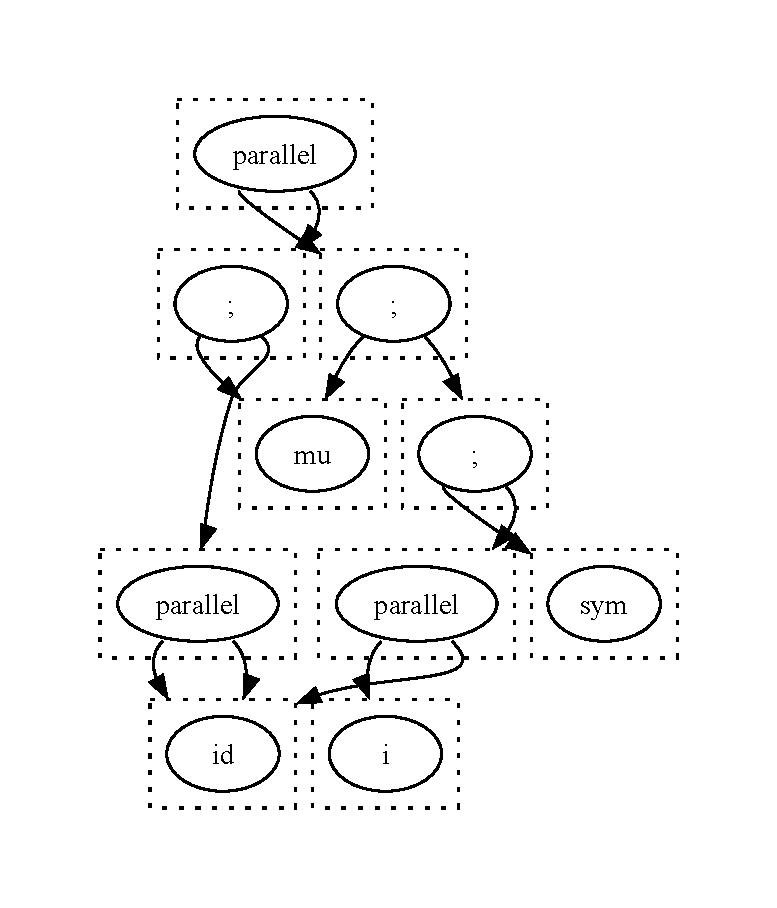
\includegraphics[scale=0.4]{figures/egraph_before_saturation.pdf}
        \end{figure}
    \end{example}
\end{frame}

\begin{frame}
    \small
    \begin{example}
        \vspace{1em}
        E-graph for
        \[
            (\mu\;;(\sigma_{1,1}\;;i \otimes id_{1})) \otimes (\mu\;;(id_{1}\otimes id_{1}))
        \]
        After saturation
        \begin{figure}
            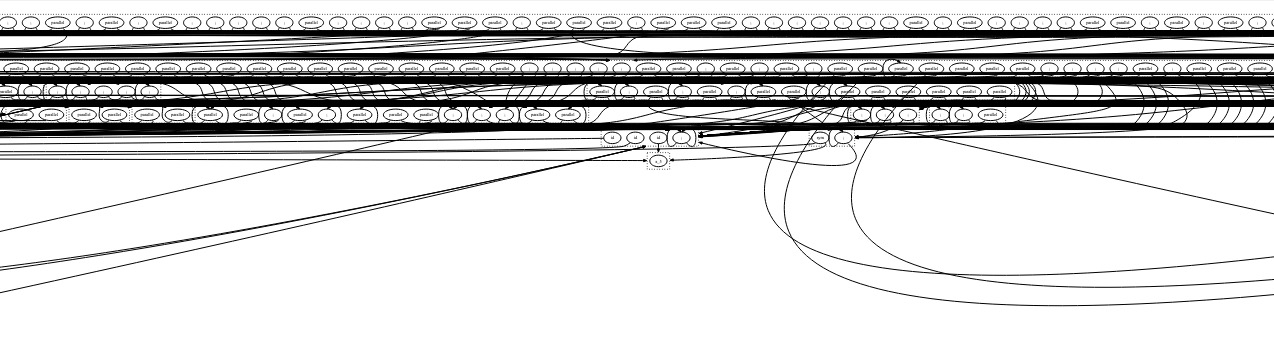
\includegraphics[width=0.9\linewidth]{figures/dot_5.jpeg}
        \end{figure}
        
        \end{example}
\end{frame}

\begin{frame}[standout]
    Can we somehow get rid of these equations?
\end{frame}

\bsubsection{String diagrams and hypergraphs}

\begin{frame}{}
    
\small

SMTs come with a two-dimensional syntax called \textit{string diagrams} which represent equivalence classes of terms quotiented by built-in equations which are a convenient tool for graphical reasoning
\[
\scalebox{0.7}{
\tikzfig{figures/string_diagrams}
}
\]

If one slides boxes along the wires or cross wires even number of times, they get the same string diagram

\end{frame}


\begin{frame}{}

    \small

    \begin{minipage}{0.6\linewidth}
        
        In particular note how bi-functoriality law gets absorbed by the notation
    \end{minipage}
    \begin{minipage}{0.35\linewidth}
        \[
         \scalebox{0.7}{
            \tikzfig{figures/bifunctoriality}
         }   
        \]        
    \end{minipage}
    \begin{minipage}{0.6\linewidth}       
        Further structure on the monoidal theory is encoded in geometrical properties on these string diagrams
    \end{minipage}
    \begin{minipage}{0.35\linewidth}

    \end{minipage}
    % \begin{minipage}{0.6\linewidth}
    %     \begin{itemize}
    %         \item There are equations for which their term-equivalent is not immediately obvious (ZX-calculus Z-spider fusion)
    %     \end{itemize}        
    % \end{minipage}
    % \begin{minipage}{0.35\linewidth}
    %     \[
    %      \scalebox{0.7}{
    %         \tikzfig{figures/Z_spider_fusion}
    %      }   
    %     \]        
    % \end{minipage}

\end{frame}

\begin{frame}
    Another benefit of string diagrams is that they simplify the additional equations for which their term-equivalent form is not immediately obvious

    \[
         \scalebox{1}{
            \tikzfig{figures/Z_spider_fusion}
         }   
    \]
\end{frame}

\begin{frame}
\vfill
Notably, string diagrams can be represented combinatorially as \alert{hypergraphs with interfaces} where the laws of the symmetric monoidal category gets \alert{absorbed} by the notion of isomorphic hypergraphs
\vfill
Diagrammatic reasoning becomes graph rewriting
\vfill
Further structure is encoded as rewrites and/or by enforcing additional constraints on the graph structure
\vfill
\end{frame}

\begin{frame}
    \begin{example}
        \begin{minipage}{0.45\linewidth}
        Assuming $\mu \coloneqq $\raisebox{-1.5em}{\scalebox{0.6}{\begin{tikzpicture}
            \begin{pgfonlayer}{nodelayer}
                \node [style=round box] (0) at (0.5, 0.5) {$\mu$};
                \node [style=none] (1) at (0.5, 1.5) {};
                \node [style=none] (2) at (0, -0.5) {};
                \node [style=none] (3) at (1, -0.5) {};
                \node [style=none] (4) at (0.25, 0.25) {};
                \node [style=none] (5) at (0.75, 0.25) {};
            \end{pgfonlayer}
            \begin{pgfonlayer}{edgelayer}
                \draw (0) to (1.center);
                \draw [bend right=15] (4.center) to (2.center);
                \draw [bend left=15] (5.center) to (3.center);
            \end{pgfonlayer}
        \end{tikzpicture}}}
        and $i \coloneqq \;\;$\raisebox{-0.2em}{\scalebox{0.6}{\begin{tikzpicture}
            \begin{pgfonlayer}{nodelayer}
                \node [style=none] (0) at (3.5, 1) {};
                \node [style=vertex] (1) at (3.5, 0.5) {};
            \end{pgfonlayer}
            \begin{pgfonlayer}{edgelayer}
                \draw (0.center) to (1);
            \end{pgfonlayer}
        \end{tikzpicture}        
        }} a string diagrammatic version of
        \[ 
            (\mu\;;(\sigma_{1,1}\;;i \otimes id_{1})) \otimes (\mu\;;(id_{1}\otimes id_{1}))
        \] looks like
    \end{minipage}
        \hfill
    \begin{minipage}{0.45\linewidth}
        \begin{tikzpicture}
                \begin{pgfonlayer}{nodelayer}
                    \node [style=round box] (0) at (0.5, 0.5) {$\mu$};
                    \node [style=none] (1) at (0.5, 1.5) {};
                    \node [style=none] (2) at (0, -0.25) {};
                    \node [style=none] (3) at (1, -0.25) {};
                    \node [style=none] (4) at (0.25, 0.25) {};
                    \node [style=none] (5) at (0.75, 0.25) {};
                    \node [style=vertex] (6) at (1, -2.25) {};
                    \node [style=none] (7) at (1, -1.75) {};
                    \node [style=round box] (8) at (3.5, 0.5) {$\mu$};
                    \node [style=none] (9) at (3.5, 1.5) {};
                    \node [style=none] (10) at (3, -0.25) {};
                    \node [style=none] (11) at (4, -0.25) {};
                    \node [style=none] (12) at (3.25, 0.25) {};
                    \node [style=none] (13) at (3.75, 0.25) {};
                    \node [style=none] (16) at (0.5, -1) {};
                    \node [style=none] (17) at (0, -1.75) {};
                    \node [style=none] (18) at (1, -1.75) {};
                    \node [style=none] (19) at (0, -2.25) {};
                    \node [style=none] (20) at (3, -2.25) {};
                    \node [style=none] (21) at (4, -2.25) {};
                \end{pgfonlayer}
                \begin{pgfonlayer}{edgelayer}
                    \draw (0) to (1.center);
                    \draw [bend right=15] (4.center) to (2.center);
                    \draw [bend left=15] (5.center) to (3.center);
                    \draw (6) to (7.center);
                    \draw (8) to (9.center);
                    \draw [bend right=15] (12.center) to (10.center);
                    \draw [bend left=15] (13.center) to (11.center);
                    \draw [in=30, out=-90] (3.center) to (16.center);
                    \draw [in=90, out=-135] (16.center) to (17.center);
                    \draw [in=315, out=90] (18.center) to (16.center);
                    \draw [in=-90, out=150] (16.center) to (2.center);
                    \draw (17.center) to (19.center);
                    \draw (10.center) to (20.center);
                    \draw (11.center) to (21.center);
                \end{pgfonlayer}
            \end{tikzpicture}
    \end{minipage}
    \vfill
    Which is already `saturated' with respect to the built-in equations
    \end{example} 
\end{frame}

\begin{frame}

A hypergraph form of the above example is 

\[
\scalebox{0.6}{
    \tikzfig{figures/hypergraph_with_interfaces}
}    
\]
    
\end{frame}

\begin{frame}[standout]
So \alert{yes}, we can get rid of these equations if we use \alert{hypergraphs} (derived from string diagrams)
\end{frame}

\begin{frame}
\vfill
The work next formalises e-graphs for SMTs that would use string diagrams (hypergraphs) as a representation for terms in a bottom-up manner deriving this formalisation from an SMT itself
\vfill
\end{frame}

% \begin{frame}{}

%     The applications of SMTs (and string diagrams) include
%     \begin{itemize}
%         \item Quantum computing
%         \item Probabilistic programming
%         \item Lambda calculus
%         \item Digital circuits
%         \item $\ldots$
%     \end{itemize}

%     Can we have e-graphs for such two-dimensional syntax (so that built-in equations are all absorbed rather than represented with e-classes)?

%     \pause

%     This work builds a foundation to answer the above question
% \end{frame}

\section{Underlying Theory}

\begin{frame}{}
    \vfill

    First we introduce the notion of an \textit{enriched} SMT where we can take formal joins of terms
    \[
    f_1 + \ldots +f_n, \text{\; where $f_{i} : m \to n$}    
    \]
    \vfill
    These formal joins will encode the equivalence classes, \textit{i.e.}, we will use them to express that $f_i \sim f_j$
    \vfill
    The joins are represented graphically as boxes
    \[
    \scalebox{0.8}{
        \tikzfig{figures/join_box}
    }    
    \]
\end{frame}

\begin{frame}{}
    \vfill
    Much like in e-graphs where $x \sim y$ implies $f(x) \sim f(y)$ for a functional symbol $f$ we have a notion of \textit{congruence} which is a bit more general since we have two sorts of composition
    \vfill
    These are encoded as string diagrams as well as the requirements that $+$ is an associative, commutative and idempotent operator
\end{frame}

\begin{frame}{}
    \[
        \scalebox{0.6}{
        \tikzfig{../figures/categorical-semantics/egraph-strings-equations}
        }
    \]
\end{frame}


\begin{frame}{}
\small
The non-destructive feature of rewriting with e-graphs is modelled by using the idempotence property of $+$
\vfill
Given a rewrite rule (in a string diagrammatic form) and a source string diagram
\begin{minipage}{0.4\linewidth}
    \[
    \scalebox{1}{
    \tikzfig{figures/rewrite_example_1}
    }
    \]
\end{minipage}
\hfill
\begin{minipage}{0.4\linewidth}
    \[
    \tikzfig{figures/rewrite_example_3}
    \]
\end{minipage}

\end{frame}
% \vfill
% These equations equip a set of terms (morphisms) with the same domain and co-domain with a structure of a semilattice and hence the models of such enriched SMTs are symmetric monoidal categories enriched over a category of semilattices

\begin{frame}
    We apply the equations (and the rewrite rule above) in the following way
    \[
    \tikzfig{figures/rewrite_example_2}
    \]
\end{frame}


\begin{frame}{}
    Such extended string diagrams have a concrete combinatorial representation which we call \textit{e-hypergraphs} with interfaces


        \begin{minipage}{0.45\linewidth}
            \[
            \tikzfig{figures/boxed_sym_string}    
            \]
        \end{minipage}
        \begin{minipage}{0.05\linewidth}
            \[
                \to
            \]
        \end{minipage}
        \begin{minipage}{0.45\linewidth}
            \[
            \scalebox{0.5}{
            \tikzfig{figures/extended_cospan_example}
            }
            \]
        \end{minipage}
\end{frame}

\begin{frame}{}
    \vfill
    Now equivalence classes represent equivalent subgraphs rather than subtrees
    \pause
    \vfill
    \pause
    Such combinatorial structures are shown to be \textit{sound} and \textit{complete} for representing terms of enriched SMTs
    \vfill
    \pause
    String diagrammatic reasoning becomes e-hypergraph rewriting
    \vfill
    \pause
    The latter is defined as a \textit{double-pushout rewriting} which is a convenient framework to study properties of a rewriting system, e.g. confluence, applicability of parallel rewrites etc.
    \vfill
    \pause
    Note that they absorb the laws of symmetric monoidal category but not the structural rules for $+$
\end{frame}

\section{Case Studies}

\bsubsection{(acyclic) E-graphs are e-hypergraphs for Cartesian monoidal theories}

\begin{frame}{}
    If we consider an SMT with a copy and delete generators we get essentially an algebraic theory, the one for which e-graphs are designed

    That is, if we consider the generators (the inputs flow from bottom to top to follow the e-graphs presentation)
    \[
	\scalebox{0.7}{
  	 \tikzfig{../figures/categorical-semantics/Cartesian-equipment}
	}
    \]

    and equations

    \begin{minipage}{0.4\linewidth}
        \[
            \scalebox{0.55}{
            \tikzfig{../figures/categorical-semantics/Cartesian-theory}	
            }
            \]
    \end{minipage}
    \hfill
    \begin{minipage}{0.5\linewidth}
        \[
            \scalebox{0.55}{
            \tikzfig{../figures/categorical-semantics/Cartesian-naturality}
            }
        \]
    \end{minipage}


    We can show that our construction is indeed a generalisation of e-graphs
\end{frame}

\begin{frame}{}
    First, consider how an e-class gets translated into a string diagrammatic form

    \begin{example}
    \[
    \tikzfig{figures/e-graphs-translation-2}
    \]
    \end{example}

    A general translation can be drawn as follows
    \[
    \tikzfig{figures/e-graphs-translation}
    \]
\end{frame}

\begin{frame}{}
    \small
    This way applying equations to an e-graph can be seen as e-hypergraph rewriting

    \[
    \scalebox{0.5}{
    \tikzfig{figures/e-graphs-translation-3}
    }
    \]\footnote{[1]Willsey, M., Nandi, C., Remy Wang, Y., Flatt, O., Tatlock, Z., and Panchekha, P., “egg: Fast and Extensible Equality Saturation”, 2020.}
    Can be rendered as
    \[
        % \hspace{1.3cm}
        \scalebox{0.38}{
        \tikzfig{../figures/categorical-semantics/egraph-translation-step-by-step-a-b}
        }
    \]
\end{frame}

\begin{frame}
    \vfill
    This serves as a sanity check for our construction, provides a categorical presentation of e-graphs and therefore a possible framework for reasoning about them in terms of e-hypergraph rewriting
    \vfill
\end{frame}

\bsubsection{Support for binding}

\begin{frame}{}
    \small
    \vfill
    Lambda calculus is a model for a Cartesian Closed SMT and the benefits of using string diagrams for lambda calculus is that they are automatically quotiented by $\alpha$-equivalence (variables just become wires) and by linear substitution
    \vfill
    Compare the following

    \begin{minipage}{0.3\linewidth}
        \[
        \scalebox{0.5}{
        \tikzfig{figures/e-graphs-binding-example-plain}
        }
        \]
    \end{minipage}
    \hfill
    \begin{minipage}{0.3\linewidth}
        \[
        \scalebox{0.5}{
        \tikzfig{figures/e-graphs-binding-example-indices}
        }
        \]
    \end{minipage}
    \hfill
    \begin{minipage}{0.3\linewidth}
        \[
        \scalebox{0.5}{
        \tikzfig{figures/e-graphs-binding-string}
        }
        \]
    \end{minipage}
    \vfill
    
\end{frame}

\begin{frame}
    \vfill
    Thus we can represent e-graphs for lambda calculus with string diagrams for an enriched Cartesian Closed SMT
    \vfill
\end{frame}

\begin{frame}
    \[
        % \hspace{1.3cm}
        \scalebox{0.4}{
        \tikzfig{../figures/categorical-semantics/e-graph-substitution}
        }
    \]
    \tiny{[2]\href{https://pldi23.sigplan.org/details/egraphs-2023-papers/12/Optimizing-Beta-Reduction-in-E-Graphs}{Optimizing-Beta-Reduction-in-E-Graphs}}
    \[
        % \hspace{1.3cm}
        \scalebox{0.35}{
        \tikzfig{../figures/categorical-semantics/e-string-substitution-2}
        }
    \]
\end{frame}

\section{Conclusion}

\begin{frame}{}
    \begin{minipage}{0.65\linewidth}
    \small
    \vfill
    \begin{itemize}
        \item We have presented a generalisation of e-graphs for SMTs which could broaden the area of application of e-graphs to
        \vfill
        \begin{itemize}
            \item Quantum processes
            \vfill
            \item Probabilistic programming
            \vfill
            \item Digital circuits
        \end{itemize}
        \vfill
        \item It also has benefits for algebraic theories like lambda calculus
        \vfill
        \item As a bonus we have a framework for reasoning about e-graphs in terms of graph rewriting
        \vfill
        \item We \textbf{did not} study the implementation of e-hypergraphs as a data structure and the corresponding equality saturation procedure
    \end{itemize}
\end{minipage}
\begin{minipage}{0.3\linewidth}
    \small
    
\includegraphics[width=\linewidth]{figures/arxiv_qr}
    Link to a pre-print$\;\uparrow$\\

    Email for collaboration:\\
    \alert{\url{axt257@student.bham.ac.uk}}
\end{minipage}
\end{frame}

\end{document}